% Created 2011-04-27 Wed 13:53

\documentclass[english,10pt,presentation]{beamer}
\usepackage[english]{babel}
\usepackage[utf8]{inputenc}
\usepackage[T1]{fontenc}
\mode<article>
{
  \usepackage{times}
  \usepackage{mathptmx}
  \usepackage[left=1.5cm,right=6cm,top=1.5cm,bottom=3cm]{geometry}
}
\usepackage{fancybox}
\usepackage{multimedia}
\usepackage{colortbl}
\usepackage{yfonts}
\usepackage{colortbl}
\usepackage{translator}
\usepackage{times}
\usepackage{fixltx2e}
\usepackage{graphicx}
\usepackage{longtable}
\usepackage{float}
\usepackage{wrapfig}
\usepackage{soul}
\usepackage{textcomp}
\usepackage{marvosym}
\usepackage{wasysym}
\usepackage{latexsym}
\usepackage{amssymb}
\usepackage{amsmath}
\usepackage{amsfonts}
\usepackage{ifthen}
\usepackage{mypgf}
\usepackage{hyperref}

\usepackage{fixltx2e}
\usepackage{graphicx}
\usepackage{longtable}
\usepackage{float}
\usepackage{wrapfig}
\usepackage{soul}
\usepackage{textcomp}
\usepackage{marvosym}
\usepackage{wasysym}
\usepackage{latexsym}
\usepackage{amssymb}
\usepackage{amsmath}
\usepackage{amsfonts}
\usepackage{ifthen}
\usepackage{hyperref}
\usepackage{mypgf}
\usepackage{algorithmic}
\usepackage{algorithm}
\providecommand{\alert}[1]{\textbf{#1}}

\title{Implementation of Contracting Curve Density Algorithm for Applications in Personal Robotics}
\author{Shulei Zhu}
\date{\today}

\usetheme{dimilar}\usecolortheme{rose}
\begin{document}

\maketitle

\begin{frame}
\frametitle{Outline}
\setcounter{tocdepth}{2}
\tableofcontents
\end{frame}

\section{Motivation}
\label{sec-1}
\begin{frame}
\frametitle{Motivation}
\label{sec-1_1}
\begin{alertblock}{Some challenging tasks in personal robotics}
\label{sec-1_1_1}
\begin{itemize}

\item Image segmentation\\
\label{sec-1_1_1_1}%
\item Pose estimation\\
\label{sec-1_1_1_2}%
\item Object recognition and tracking\\
\label{sec-1_1_1_3}%
\end{itemize} % ends low level
\end{alertblock}
\begin{block}{Model-base method}
\label{sec-1_1_2}
\begin{itemize}

\item require much information external to the image\\
\label{sec-1_1_2_1}%
\item Curve-fitting: a crucial part of these problems\\
\label{sec-1_1_2_2}%
\end{itemize} % ends low level
\end{block}
\begin{exampleblock}{Requirements}
\label{sec-1_1_3}
\begin{itemize}

\item Robustness: stable even in the presence of heavy texture, clutter, poor contrast, partial occlusion\\
\label{sec-1_1_3_1}%
\item Accuracy: high sub-pixel accuracy\\
\label{sec-1_1_3_2}%
\item Efficiency: time-constrained, limited computer hardware resources in personal robotics\\
\label{sec-1_1_3_3}%
\end{itemize} % ends low level
\end{exampleblock}
\end{frame}
\section{How the original CCD algorithm works?}
\label{sec-2}
\begin{frame}
\frametitle{How the original CCD algorithm works?}
\label{sec-2_1}
\begin{columns}
\begin{column}{0.4\textwidth}
\begin{exampleblock}{Flowchart of the CCD algorithm}
\label{sec-2_1_1}

   \begin{figure}[htb]
   \centering
   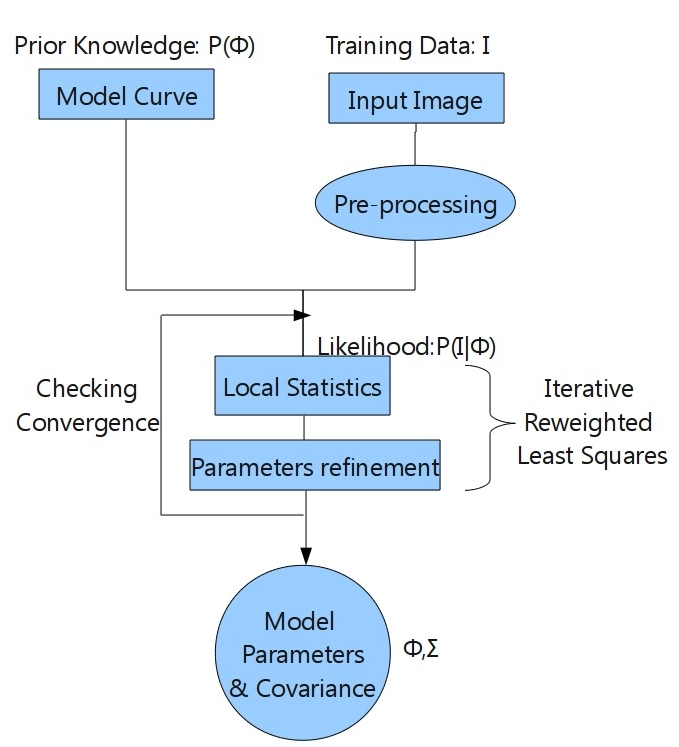
\includegraphics[width=4cm,angle=0]{./flowchart.jpg}
   \caption{\label{fig: flowchart}the CCD algorithm}
   \end{figure}
\end{exampleblock}
\end{column}
\begin{column}{0.6\textwidth}
\begin{exampleblock}{Basic steps of the CCD algorithm}
\label{sec-2_1_2}

\begin{enumerate}
\item <1-> Contour initialization : initialize the model parameter vector
$\Phi$ (6-DOF or 8-DOF) and covariance matrix $\Sigma_{\Phi}$
\item <2-> Learning of local statistics : evaluate the likelihood; build
the cost function 
\item <3-> Refinement of model parameters : Maximize the cost function
using optimization algorithms
\item <4-> Check for convergence, if not, go to Step 2
\end{enumerate}
\end{exampleblock}
\end{column}
\end{columns}
\end{frame}
\begin{frame}
\frametitle{Sketch of the CCD algorithm}
\label{sec-2_2}

     \begin{figure}[htb]
     \centering
     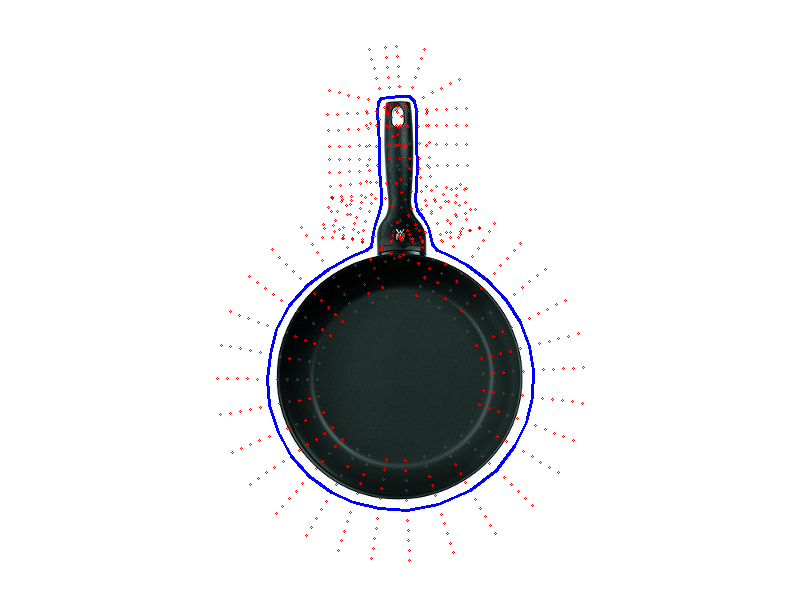
\includegraphics[width=6cm,angle=0]{./pan_contour.jpg}
     \caption{\label{fig:contour}The contour of a pan}
     \end{figure}
\end{frame}
\begin{frame}
\frametitle{An alternative view of the CCD algorithm}
\label{sec-2_3}
\begin{exampleblock}{A classification problem}
\label{sec-2_3_1}

    \begin{figure}[htb]
    \centering
    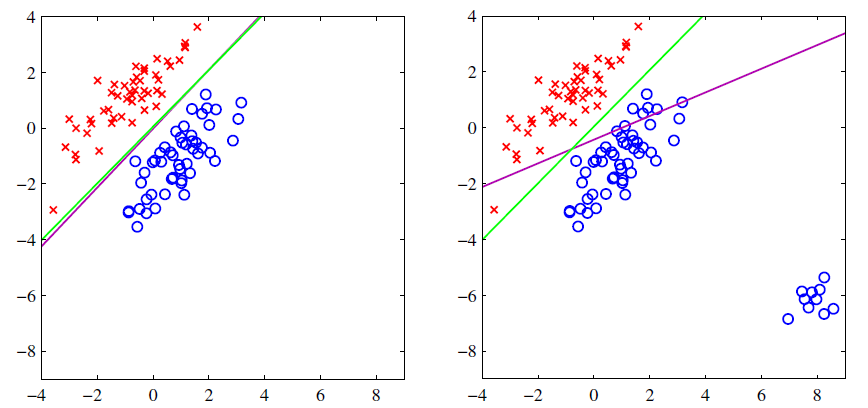
\includegraphics[width=7cm,angle=0]{./classification.png}
    \caption{\label{fig:class}A classification problem   \cite{prml}}
    \end{figure}
\end{exampleblock}
\end{frame}
\begin{frame}
\frametitle{An alternative view of the CCD algorithm}
\label{sec-2_4}
\begin{exampleblock}{Probit regression}
\label{sec-2_4_1}
\begin{itemize}

\item Evaluation of conditional distribution $p(\Phi|\mathbf{I})$
\label{sec-2_4_1_1}%
\begin{displaymath}
p(\Phi|\mathbf{I})
\propto \underbrace{p(\mathbf{I}|\mathbf{m}_{\Phi},
\Sigma_{\Phi})}_{\mathrm{local\ statistics}}\quad\times\quad
\underbrace{p(\Phi)}_{\mathrm{prior\ distribution}}
\end{displaymath}
Local statistics (likelihood): a probit function with
respect to $\Phi$

\item Goal: MAP (maximum a posteriori probability) solution of cost function $\mathcal{Q}(\Phi)$
\label{sec-2_4_1_2}%
\begin{displaymath}
\mathcal{Q}(\Phi) = \underset{\Phi}{\arg\max}\ \mathrm{ln}(p(\Phi|\mathbf{I}))
\end{displaymath}
Approach: iterative reweighted least  squares (IRLS) e.g. Gaussian
Newton method, Gradient decent and SVM Least Squares.

\end{itemize} % ends low level
\end{exampleblock}
\end{frame}
\section{Improvements of the original algorithm}
\label{sec-3}
\begin{frame}
\frametitle{Quadratic and Cubic B-spline curves}
\label{sec-3_1}
\begin{exampleblock}{B-spline curves}
\label{sec-3_1_1}

\begin{equation*}
  \mathbf{C}(u) =  \sum_{i=0}^{m-n-2} P_{i} B_{i,n}(u) \mbox{ , } u \in [u_{n},u_{m-n-1}]
\end{equation*}
\begin{figure}[htb]
\centering
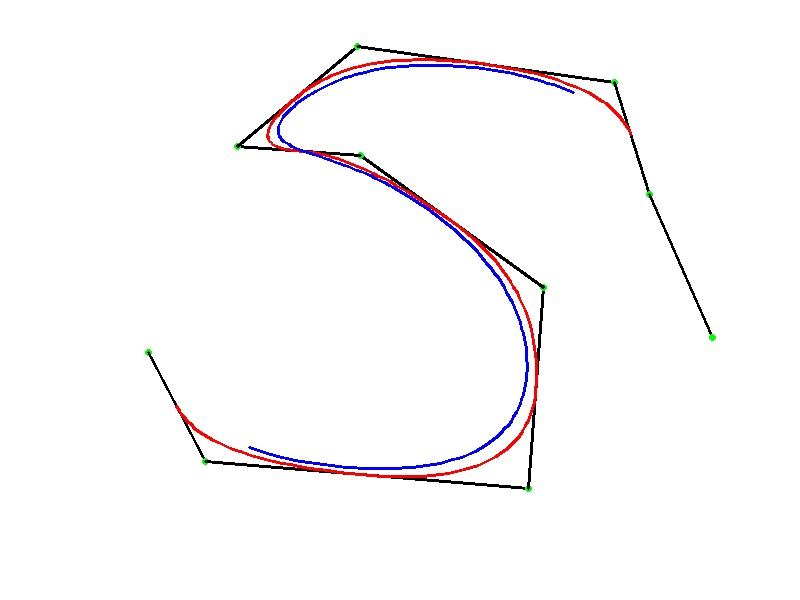
\includegraphics[width=6cm,angle=0]{./bspline.jpg}
\caption{\label{fig: bspline}B-spline curves of degree = 1, 2, 3}
\end{figure}
\end{exampleblock}
\end{frame}
\begin{frame}
\frametitle{Logistic and Probit function}
\label{sec-3_2}
\begin{columns}
\begin{column}{0.5\textwidth}
\begin{exampleblock}<1->{Logistic function}
\label{sec-3_2_1}

    \begin{figure}[htb]
    \centering
    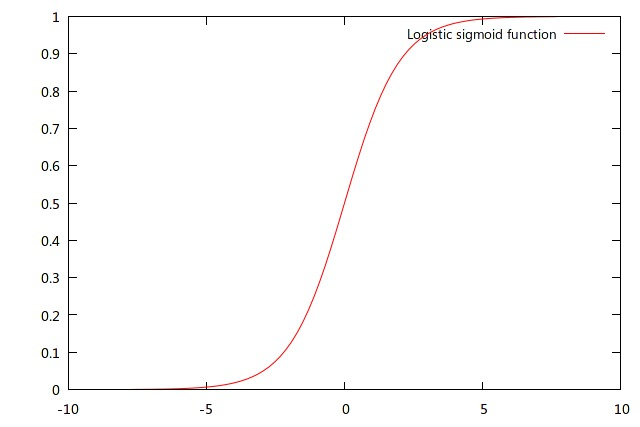
\includegraphics[width=4cm,angle=0]{./logistic.jpg}
    \caption{\label{fig:log}Logistic function}
    \end{figure}
\begin{displaymath}
f(\cdot) = \frac{1}{1+\mathrm{e}^{-x}}
\end{displaymath}
\end{exampleblock}
\end{column}
\begin{column}{0.5\textwidth}
\begin{exampleblock}<2->{Probit function}
\label{sec-3_2_2}

    \begin{figure}[htb]
    \centering
    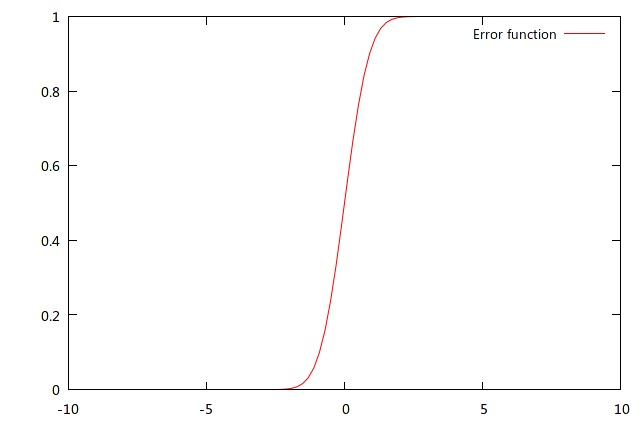
\includegraphics[width=4cm,angle=0]{./erf.jpg}
    \caption{\label{fig: probit}Probit function}
    \end{figure}
\begin{displaymath}
f(\cdot) = \frac{1}{2}(\frac{1}{\sqrt{2}}erf(x) + 1)
\end{displaymath}
\end{exampleblock}
\end{column}
\end{columns}
\end{frame}
\begin{frame}
\frametitle{Logistic and Probit function}
\label{sec-3_3}

    \begin{figure}[htb]
    \centering
    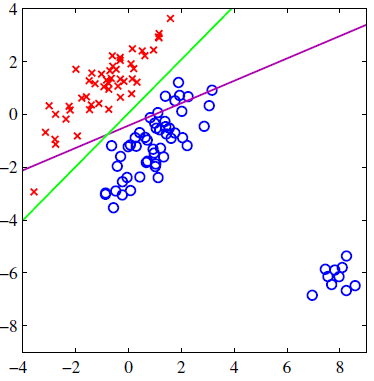
\includegraphics[width=7cm,angle=0]{./outliers.png}
    \caption{\label{fig:class}Probit function is highly sensitive for outliers \cite{prml}}
    \end{figure}
\end{frame}
\begin{frame}
\frametitle{Three-dimensional Affine Shape-space}
\label{sec-3_4}
\begin{columns}
\begin{column}{0.5\textwidth}
\begin{block}{Parallax effect in two-dimensional affine shape-space}
\label{sec-3_4_1}

    \begin{figure}[htb]
    \centering
    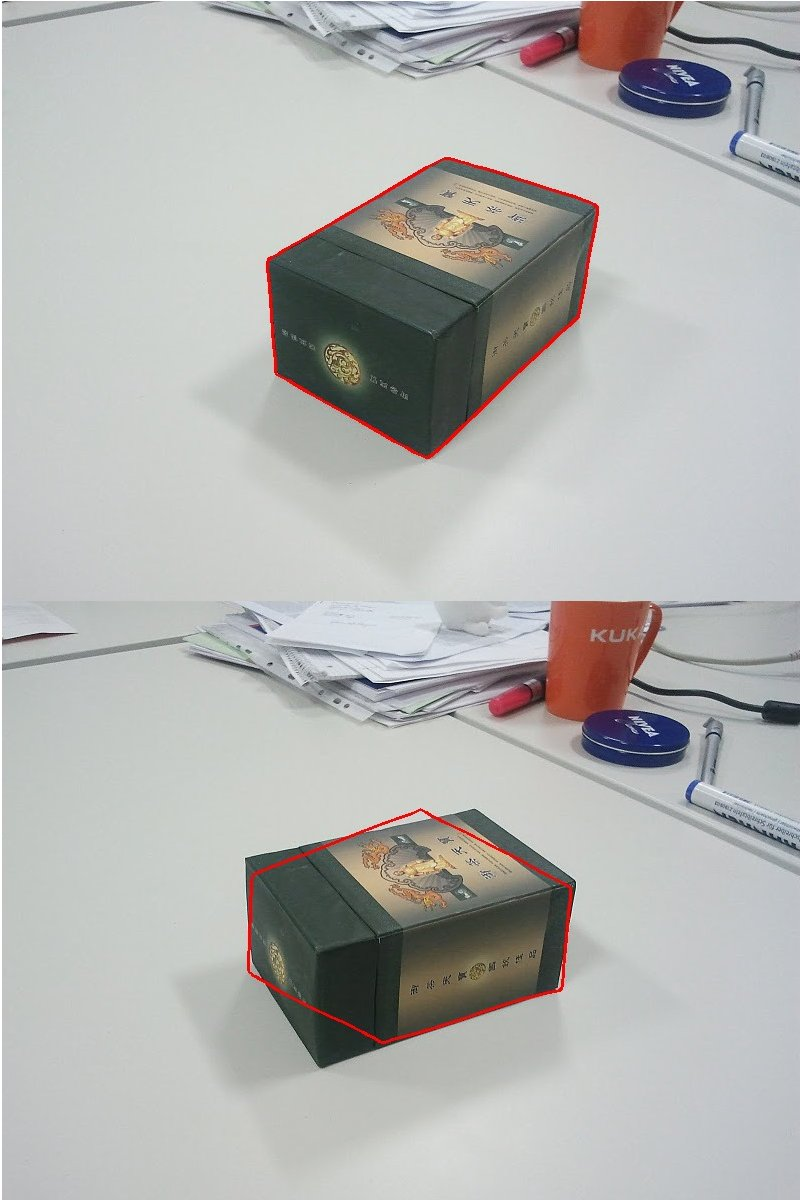
\includegraphics[width=3cm,angle=0]{./planar.jpg}
    \caption{\label{fig:parallax effect}Parallax effect}
    \end{figure}
\end{block}
\end{column}
\begin{column}{0.5\textwidth}
\begin{block}{Three-dimensional affine shape-space}
\label{sec-3_4_2}

    \begin{figure}[htb]
    \centering
    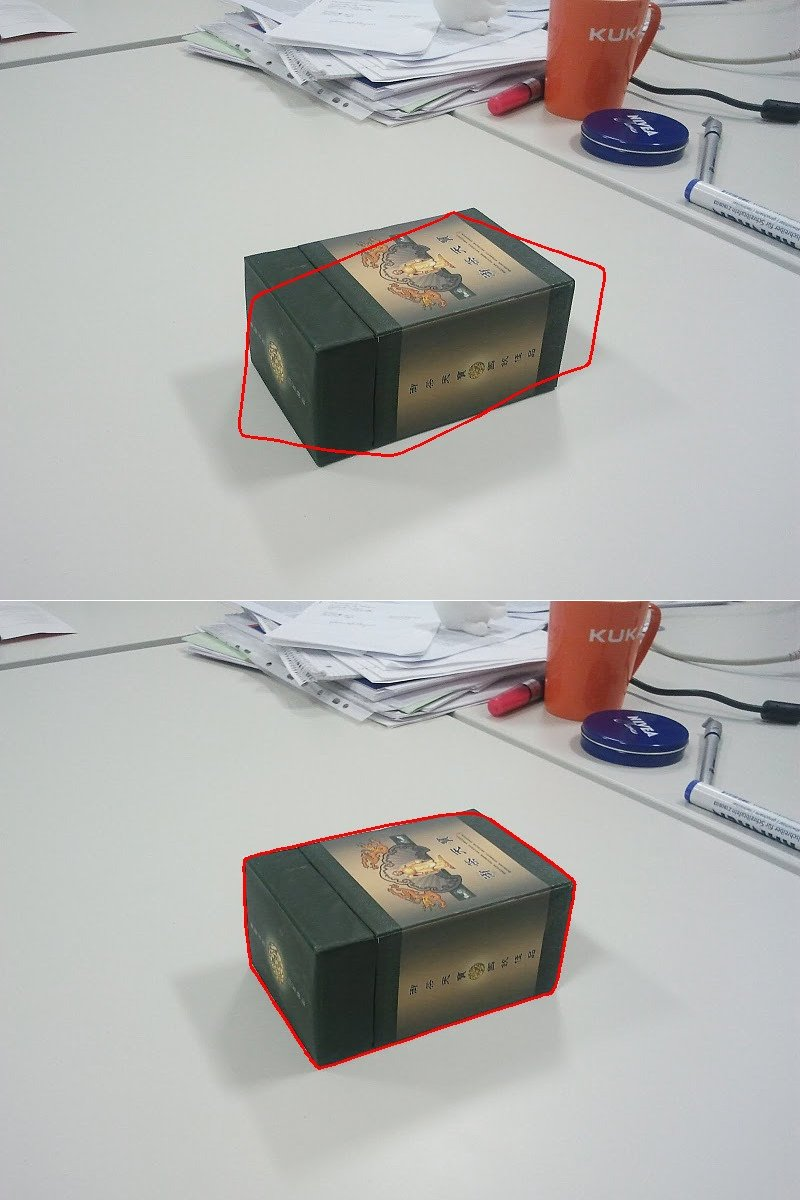
\includegraphics[width=3cm,angle=0]{./nonplanar.jpg}
    \caption{\label{fig:3das}Three-dimensional affine shape-space}
    \end{figure}
\end{block}
\end{column}
\end{columns}
\end{frame}
\begin{frame}
\frametitle{Automated initialization methods (I)}
\label{sec-3_5}
\begin{block}{Initialization from SIFT Features}
\label{sec-3_5_1}

    \begin{figure}[htb]
    \centering
    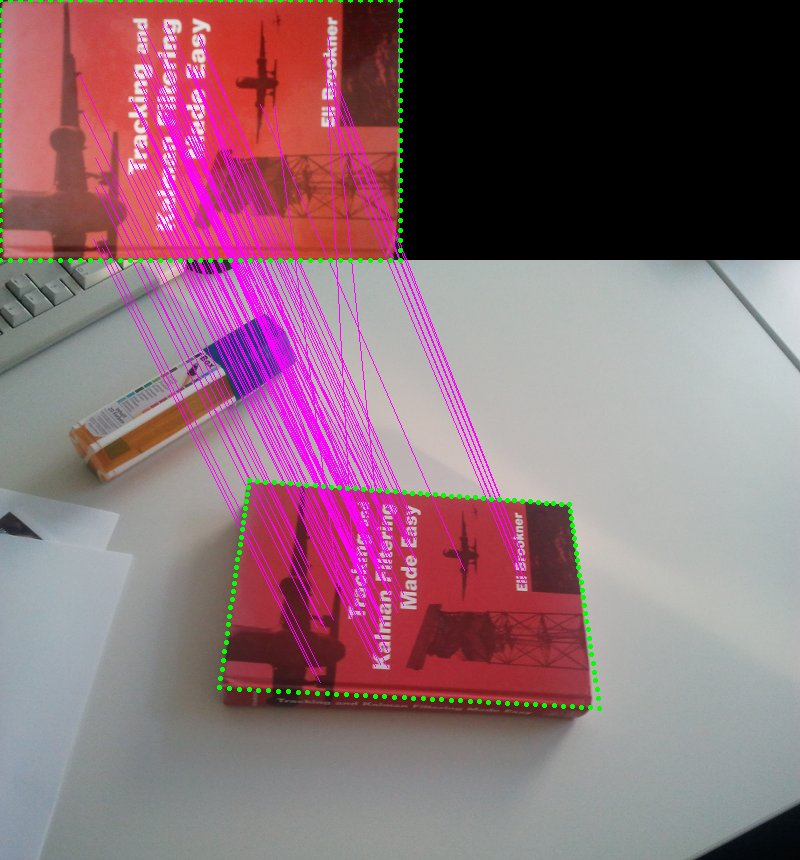
\includegraphics[width=6cm,angle=0]{./sift.jpg}
    \caption{\label{fig:sift}Initialization from SIFT Features}
    \end{figure}
\end{block}
\end{frame}
\begin{frame}
\frametitle{Automated initialization methods (II)}
\label{sec-3_6}
\begin{block}{Initialization from projection of point clouds onto the image}
\label{sec-3_6_1}

    \begin{figure}[htb]
    \centering
    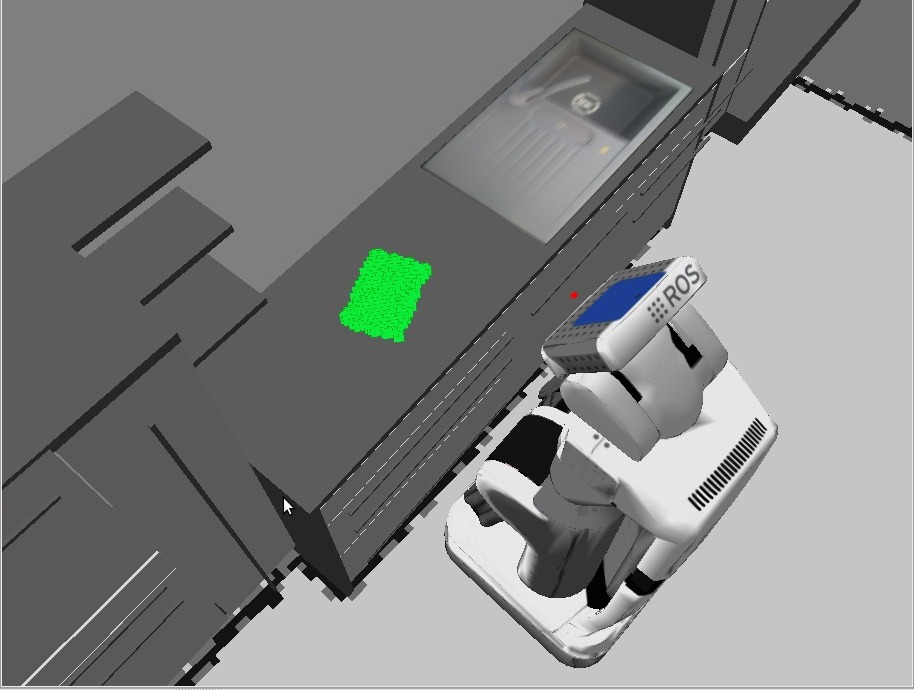
\includegraphics[width=6cm,angle=0]{./pr2b.jpg}
    \caption{\label{fig:sift}Initialization from projection of point clouds onto the image}
    \end{figure}
\end{block}
\end{frame}
\section{The CCD tracker}
\label{sec-4}
\begin{frame}
\frametitle{Contracting Curve Density (CCD) Tracker}
\label{sec-4_1}

  \begin{algorithm}[H]
    \caption{Contracting Curve Density (CCD) tracker}
    \begin{algorithmic}[1]
      \STATE $\Phi \gets 0$
      \STATE $\mathbf{C} \gets contour\_initialization()$
      \WHILE{$NewFrame$}
        \STATE $ \mathbf{I} \gets pre\_processing()$
        \STATE $ \mathbf{C} \gets contour\_distortion(\Phi)$
        \STATE $\Sigma \gets covariance\_initialization()$
        \STATE $\Phi \gets \Phi^{\mathrm{old}}$
        \WHILE{$convergence = FALSE$}
          \STATE $local\_statistics\_learning() $
          \STATE $cost\_function\_MAP() $
        \ENDWHILE
        \STATE $\Phi \gets \Phi_{MAP}$
        \STATE $\Sigma \gets \Sigma_{MAP}$
      \ENDWHILE
    \end{algorithmic}
  \end{algorithm}
\end{frame}
\section{Results of the Experiments}
\label{sec-5}
\begin{frame}
\frametitle{Segmentation}
\label{sec-5_1}

   \begin{figure}[htb]
   \centering
   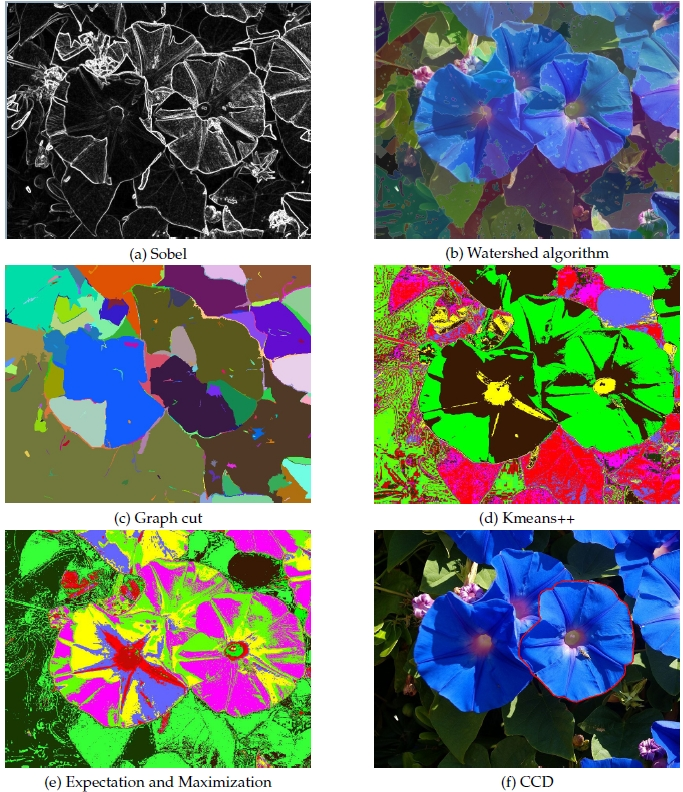
\includegraphics[width=6cm,angle=0]{./segmentation.jpg}
   \caption{\label{fig:seg}A Comparison of Image Segmentation Algorithms}
   \end{figure}
\end{frame}
\begin{frame}
\frametitle{Manual initialization}
\label{sec-5_2}
\begin{alertblock}{Shadow effects}
\label{sec-5_2_1}

    \begin{figure}[htb]
    \centering
    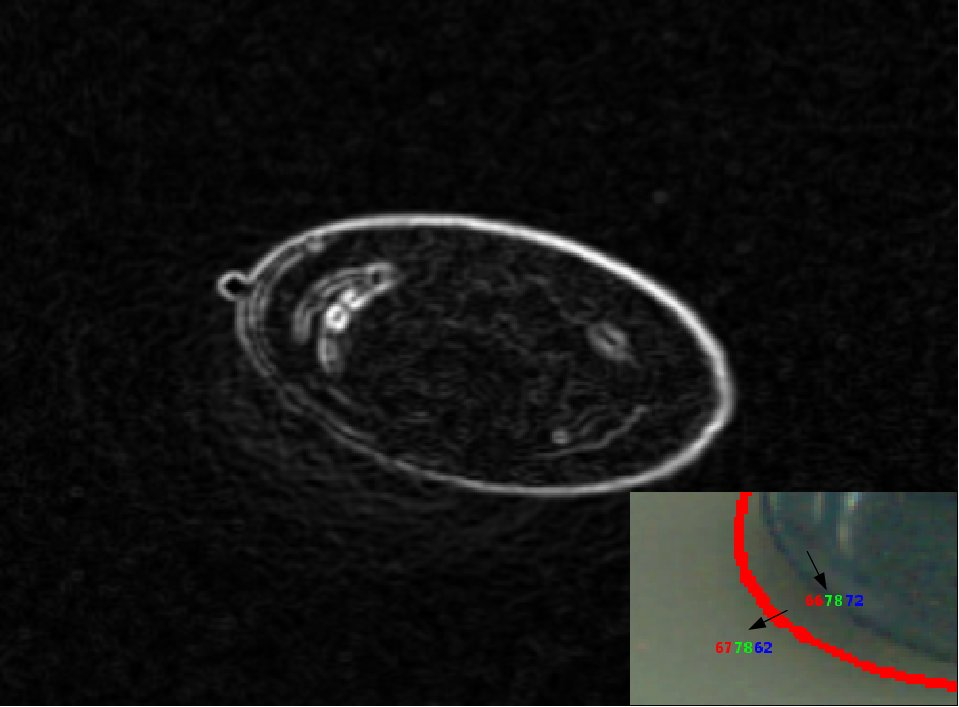
\includegraphics[width=8cm,angle=0]{./edge.jpg}
    \caption{\label{fig:shadow}Shadow effects}
    \end{figure}
\end{alertblock}
\end{frame}
\begin{frame}
\frametitle{Initialization from SIFT Features}
\label{sec-5_3}
\begin{exampleblock}{Tracking initialized from SIFT features}
\label{sec-5_3_1}
\begin{itemize}

\item Match SIFT keypoints between the template image and the test image\\
\label{sec-5_3_1_1}%
\item Discard the false matching points using the RANSAC algorithm\\
\label{sec-5_3_1_2}%
\item Compute the homography\\
\label{sec-5_3_1_3}%
\item Transform the contour of the template image onto the test image\\
\label{sec-5_3_1_4}%
\item Apply the CCD tracker to the video\\
\label{sec-5_3_1_5}%
\end{itemize} % ends low level
\end{exampleblock}
\end{frame}
\section{Summary and Future work}
\label{sec-6}
\begin{frame}
\frametitle{Summary}
\label{sec-6_1}
\begin{block}{Investigate and implement the CCD approach}
\label{sec-6_1_1}
\begin{itemize}

\item Based on the OpenCV\\
\label{sec-6_1_1_1}%
\item A ROS package: provide a ROS node interface to the ccd class\\
\label{sec-6_1_1_2}%
\url{http://www.ros.org/wiki/contracting-curve-density}

\item Released under open source BSD license\\
\label{sec-6_1_1_3}%
\end{itemize} % ends low level
\end{block}
\begin{block}{Improvements}
\label{sec-6_1_2}
\begin{itemize}

\item B-spline curve and three-dimensional affine shape-space\\
\label{sec-6_1_2_1}%
\item Logistic regression\\
\label{sec-6_1_2_2}%
\item Automated contour initialization methods: SIFT features and point clouds\\
\label{sec-6_1_2_3}%
\end{itemize} % ends low level
\end{block}
\end{frame}
\begin{frame}
\frametitle{Future work}
\label{sec-6_2}
\begin{exampleblock}{Future work}
\label{sec-6_2_1}
\begin{itemize}

\item Use statistics based on other image features instead of the RGB statistics\\
\label{sec-6_2_1_1}%
\item Integration of the CCD algorithm into a more complex tracking framework (e.g. the Lucas-Kanade method (LKM), the extended Kalman  filter (EKF))\\
\label{sec-6_2_1_2}%
\item B-spline can not precisely represent many useful simple curves such as circles and ellipses, thus, Non-uniform rational B-spline (NURBS) is required for the CCD algorithm.\\
\label{sec-6_2_1_3}%
\item Port to Android system to support mobile applications\\
\label{sec-6_2_1_4}%
\item \ldots{}.\\
\label{sec-6_2_1_5}%
\end{itemize} % ends low level
\end{exampleblock}
\end{frame}
\begin{frame}
\frametitle{Thank you}
\label{sec-6_3}

\setbeamercolor{bgcolor}{fg=black,bg=blue!50}
\begin{beamercolorbox}[rounded=true, shadow=true, wd=10cm]{bgcolor}
\label{sec-6_3_1}

\begin{center}
\large Thank you for your attention!
\end{center}
\end{beamercolorbox}
\end{frame}
\begin{frame}
\frametitle{References}
\label{sec-6_4}

\begin{thebibliography}{10}
\bibitem{prml}[Bishop, 2006]
Christopher M. Bishop
  \newblock Pattern recognition and machine learning
\end{thebibliography}
\end{frame}

\end{document}
